\section{MaterialGAN: A Generative SVBRDF Model}
\label{sec:svbrdf:gan}

Generative Adversarial Networks \cite{goodfellow2014generative} are trained to map an input from a latent space (often randomly sampled from a multi-variate normal distribution) to a plausible instance of the target distribution.
In recent years, GANs have made remarkable progress in synthesizing high-resolution, photo-realistic images. Inspired by this progress, we propose MaterialGAN, a GAN that is trained to generate plausible materials, thus implicitly learning an SVBRDF manifold. MaterialGAN is based on the architecture of StyleGAN2 \cite{karras2020analyzing}.


\subsection{Overview of StyleGAN and its latent spaces}
\label{ssec:latent_space}

StyleGAN2 \cite{karras2020analyzing} is an improvement of StyleGAN \cite{karras2019style} and is the state-of-the-art generative adversarial network (GAN) for image synthesis, especially for human faces.
The architecture has several advantages over previous models like ProgressiveGAN \cite{karras2018progressive} and DCGAN \cite{radford2015unsupervised}. For our purposes, the main advantage is that the model is not simply a black-box stack of convolution and upsampling layers, but has additional, more specific structure, allowing for much easier inversion (latent space optimization).
The StyleGAN2 architecture starts with a learned constant $4 \times 4 \times 512$ tensor and progressively upsamples it to the final output target resolution via a sequence of convolutional and upsampling layers (7 in total to end with a final image resolution of $256 \times 256$).
Given an input latent code vector $\bmz \in \calZ \subset \bbR^{512}$, StyleGAN2 transforms it through a non-linear mapping network of fully-connected layers into an intermediate latent vector $\bmw \in \calW \subset \bbR^{512}$.
The rationale for the introduction of the space of~$\calW$ is that while $\calZ$ requires (almost) every latent $\bmz \in \calZ$ to correspond to a realistic output, vectors $\bmw \in \calW$ are free from this overly stringent constraint, which leads to a less ``entangled'' mapping, with more meaningful dimensions (see \cite{karras2019style,karras2020analyzing} for more discussion).
In the original StyleGAN, the vector $\bmw \in \calW$ is mapped via a learned affine transformation to mean and variance ``style'' vectors that control adaptive instance normalizations (AdaIN) \cite{huang2017arbitrary} that are applied before and after every convolution in the generation process (thus $7 \times 2 = 14$ times for a model of resolution $256 \times 256$). The statistics of the AdaIN normalizations caused the feature maps and output images of StyleGAN to suffer from droplet artifacts. StyleGAN2 removes the droplet artifacts entirely by replacing the AdaIn normalization layers with a demodulation operation which bakes the entire style block into a single layer while maintaining the same scale-specific control as StyleGAN.
We construct a matrix $\bmw^+ \in \calW^+ \subset \bbR^{512 \times 14}$ by replicating $\bmw$ 14 times.
During training and standard synthesis, the columns of $\bmw^+$ are identical, and correspond to $\bmw$.
However, as we will discuss later (and similar to Abdal et al. \cite{abdal2019image2stylegan}), we relax this constraint when optimizing for an embedding; $\calW^+$ thus becomes an extended latent space, more powerful than $\calW$ or $\calZ$.
Additionally, StyleGAN2 injects Gaussian noise, $\bmxi$, into each of the 14 layers of the generator.
This noise gives StyleGAN2 the ability to synthesize stochastic details at multiple resolutions.
Abdal et al. \cite{abdal2020image2stylegan++} make the observation that one can also treat these noise inputs $\bmxi$ as a latent space $\calN$. Thus, combining these two spaces defines yet another latent space $\calWN$.


\subsection{MaterialGAN training}
\label{ssec:training}

MaterialGAN was trained with the dataset provided by Deschaintre et al. \cite{deschaintre2018single} (and also used in Gao et al. \cite{gao2019deep}). They generated this dataset by sampling the parameters of procedural material graphs from Allegorithmic Substance Share to create an initial set of 155 high-quality SVBRDFs at resolution $4096 \times 4096$. The dataset was augmented by blending multiple SVBRDFs and generating $256 \times 256$ resolution crops at random positions, scales and rotations. The final dataset consists of around 200,000 SVBRDFs. For detailed information about the curation of dataset we refer the reader to \cite{deschaintre2018single}. Since pairs of SVBRDFs in the dataset were the same with only a slight variation, we selected 100,000 SVBRDFs.
The maps for each SVBRDF are stacked in 9 channels (3 for albedo, 2 for normals, 1 for roughness, and 3 for specular albedo). We account for this by adapting the MaterialGAN architecture to output 9-channel outputs. MaterialGAN is trained in TensorFlow (version 1.15) with the same loss functions and similar hyper-parameters from StyleGAN2 \cite{karras2020analyzing}. StyleGAN2 configuration F was used for all experiments. The generator and discriminator were trained using Adam optimizers. The learning rate was increased per resolution from 0.001 to 0.0025 for both the generator and the discriminator. The discriminator was shown 25 million images. Training on 8$\times$ Nvidia Tesla V100 takes about 5 days.
Figure \ref{fig:svbrdf:matgan} shows materials generated by randomly sampling the MaterialGAN latent space and images rendered from them. As can be seen here, MaterialGAN generates a wide variety of nearly photorealistic materials ranging from structured to stochastic, diffuse to specular, and with large-scale variations to fine detail. Furthermore, Figure \ref{fig:svbrdf:morph_fake} and the accompanying video show example interpolations between pairs of generated materials in the latent space, producing plausible non-linear morphing results.

\begin{figure}[!ht]
	\centering
	\setlength{\resLen}{5.in}
	\addtolength{\tabcolsep}{0pt}
	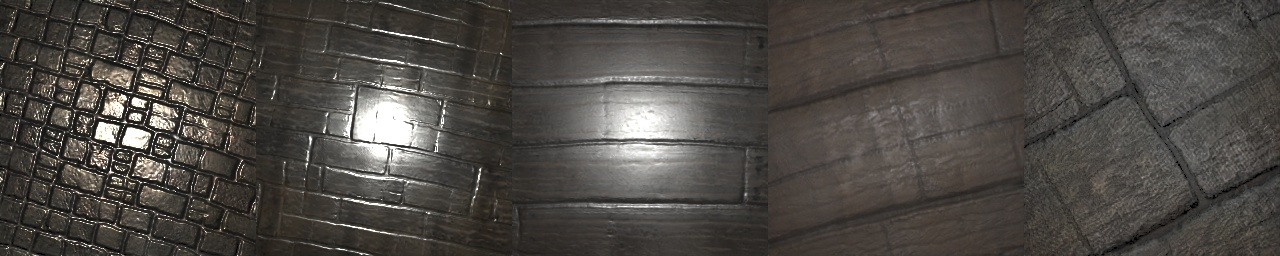
\includegraphics[width=\resLen]{svbrdf/others/interp/261_76_renders.jpg}\\[2pt]
	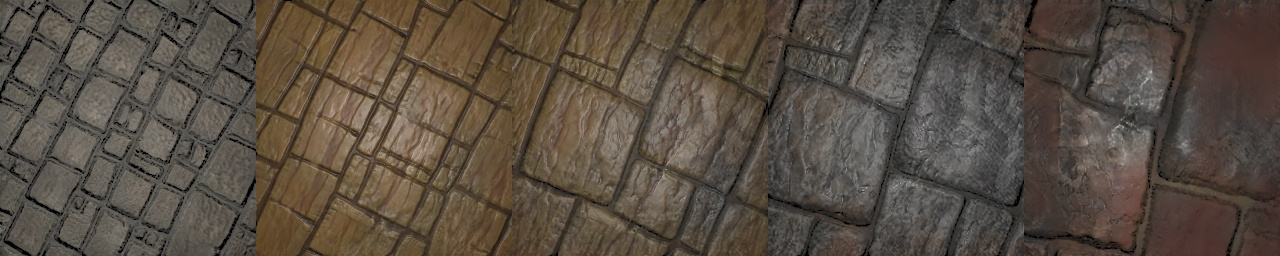
\includegraphics[width=\resLen]{svbrdf/others/interp/59_39_renders.jpg}\\[2pt]
	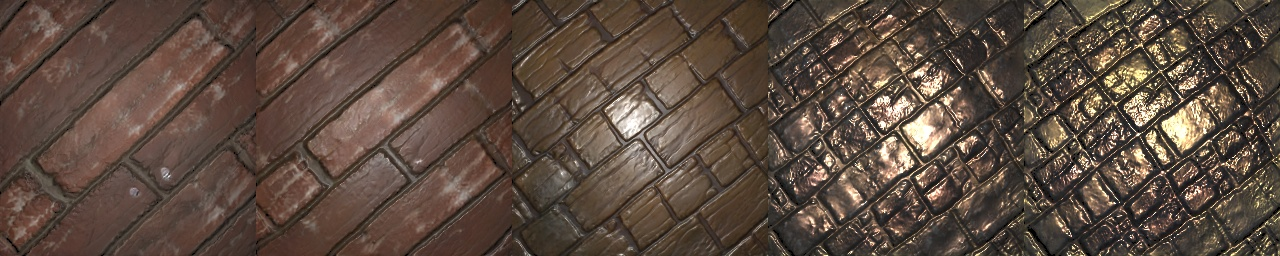
\includegraphics[width=\resLen]{svbrdf/others/interp/78_18_renders.jpg}\\[2pt]
	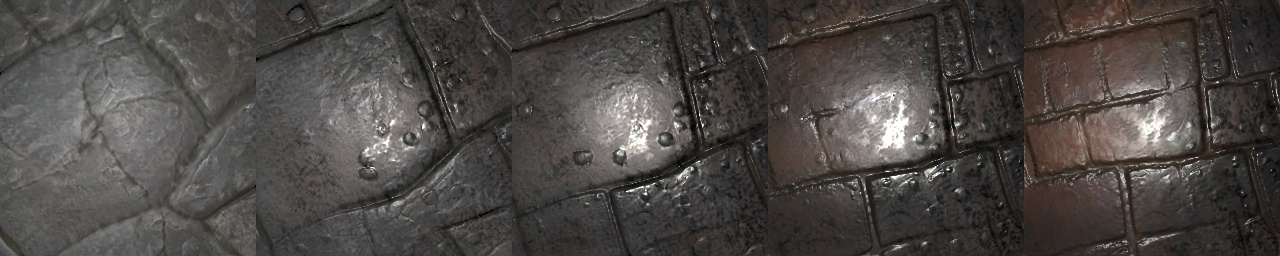
\includegraphics[width=\resLen]{svbrdf/others/interp/86_10_renders.jpg}
	\caption[Interpolation in MaterialGAN latent space]{\label{fig:svbrdf:morph_fake}
		\textbf{Interpolation in MaterialGAN latent space.} Each row shows an example of interpolation between two randomly generated materials, demonstrating non-linear morphing behavior.
	}
\end{figure}

